\title{Milestone 4}
\author{Singularity Software}
\date{\today}

\documentclass[12pt]{article}
\usepackage[a4paper]{geometry}
\usepackage{makeidx}
\usepackage{lscape}
\usepackage{amsmath}
\usepackage{graphicx}
\usepackage[final]{pdfpages}

\geometry{top=1.0in, bottom=1.0in, left=1.0in, right=1.0in} % Sets the margins

\setlength{\parindent}{0pt} % Fixes the paragraph spacing problem

\renewcommand*\arraystretch{1.5}

\begin{document}

\begin{center}
	\LARGE{Milestone 5} \\
	\Large{\textit{Singularity Software}} \\
	\vspace{.05in}
	\normalsize{\today} \\
\end{center}

\section*{Integration Testing}
Without true integration tests, we are using example applications to drive integration testing of our emulator. No one application includes each available portion of our emulator, but complete coverage is attained by testing each of the three example applications.

\begin{description}
	\item[CubeTest:]{CubeTestApp is a simple (read "not fun") game which responds to cube manipulations by changing the background color of the manipulated cube. This application exploits the following functionalities:
				\begin{itemize}
					\item{Filling background color}
					\item{Cube tilting (all four directions)}
					\item{Cube screen press}
					\item{Cube flip}
					\item{Cube shake}
					\item{Pause application event handling}
					\item{Resume application event handling}
				\end{itemize}
				}
	\item[FractionOrdering:]{FractionOrderingApp is a fun (and educational!) game that serves as an entertaining way to learn fractions. Each cube displays a unique, nonzero fraction. The player must arrange the cubes from left to right such that the fractions are in an increasing order. When they are successful at arranging two cubes relatively, they are met with a confirmation message, and when all of the cubes are ordered correctly, a reassuring vote of confidence is played. However, when cubes are placed in an incorrect order, the user is confronted with a failure message. This application exploits the following functionalities:
				\begin{itemize}
					\item{Filling background color on a cube}
					\item{Displaying images on cubes}
					\item{Playing sounds in the emulator}
					\item{Checking cube neighbors}
					\item{Drawing rectangles on the cube}
				\end{itemize}
				}
	\item[WordMaker:]{WordMakerApp is a fun (and educational!) game that serves as an entertaining way to learn new words or practice spelling. Each cube displays a letter. The player must arrange the cubes from left to right such that the letters spell out an English word. Successes and failures are met with responses like in the FractionOrderingApp. This application exploits the following functionalities:
				\begin{itemize}
					\item{Filling background color on a cube}
					\item{Displaying images on cubes}
					\item{Playing sounds in the emulator}
					\item{Checking cube neighbors}
				\end{itemize}
				}
\end{description}

These integration tests cover the major functionality of the Sifteo cubes as integrated into our emulator. Other features, like pausing/resuming, exception handling, and zooming, are tested on the emulator only and don't require integration testing with the applicaations.

\section*{Code Maintenance Plan}

\section*{Sprints 4 Backlogs}
The following pages show the backlog for the previous sprint (sprint 4). \\

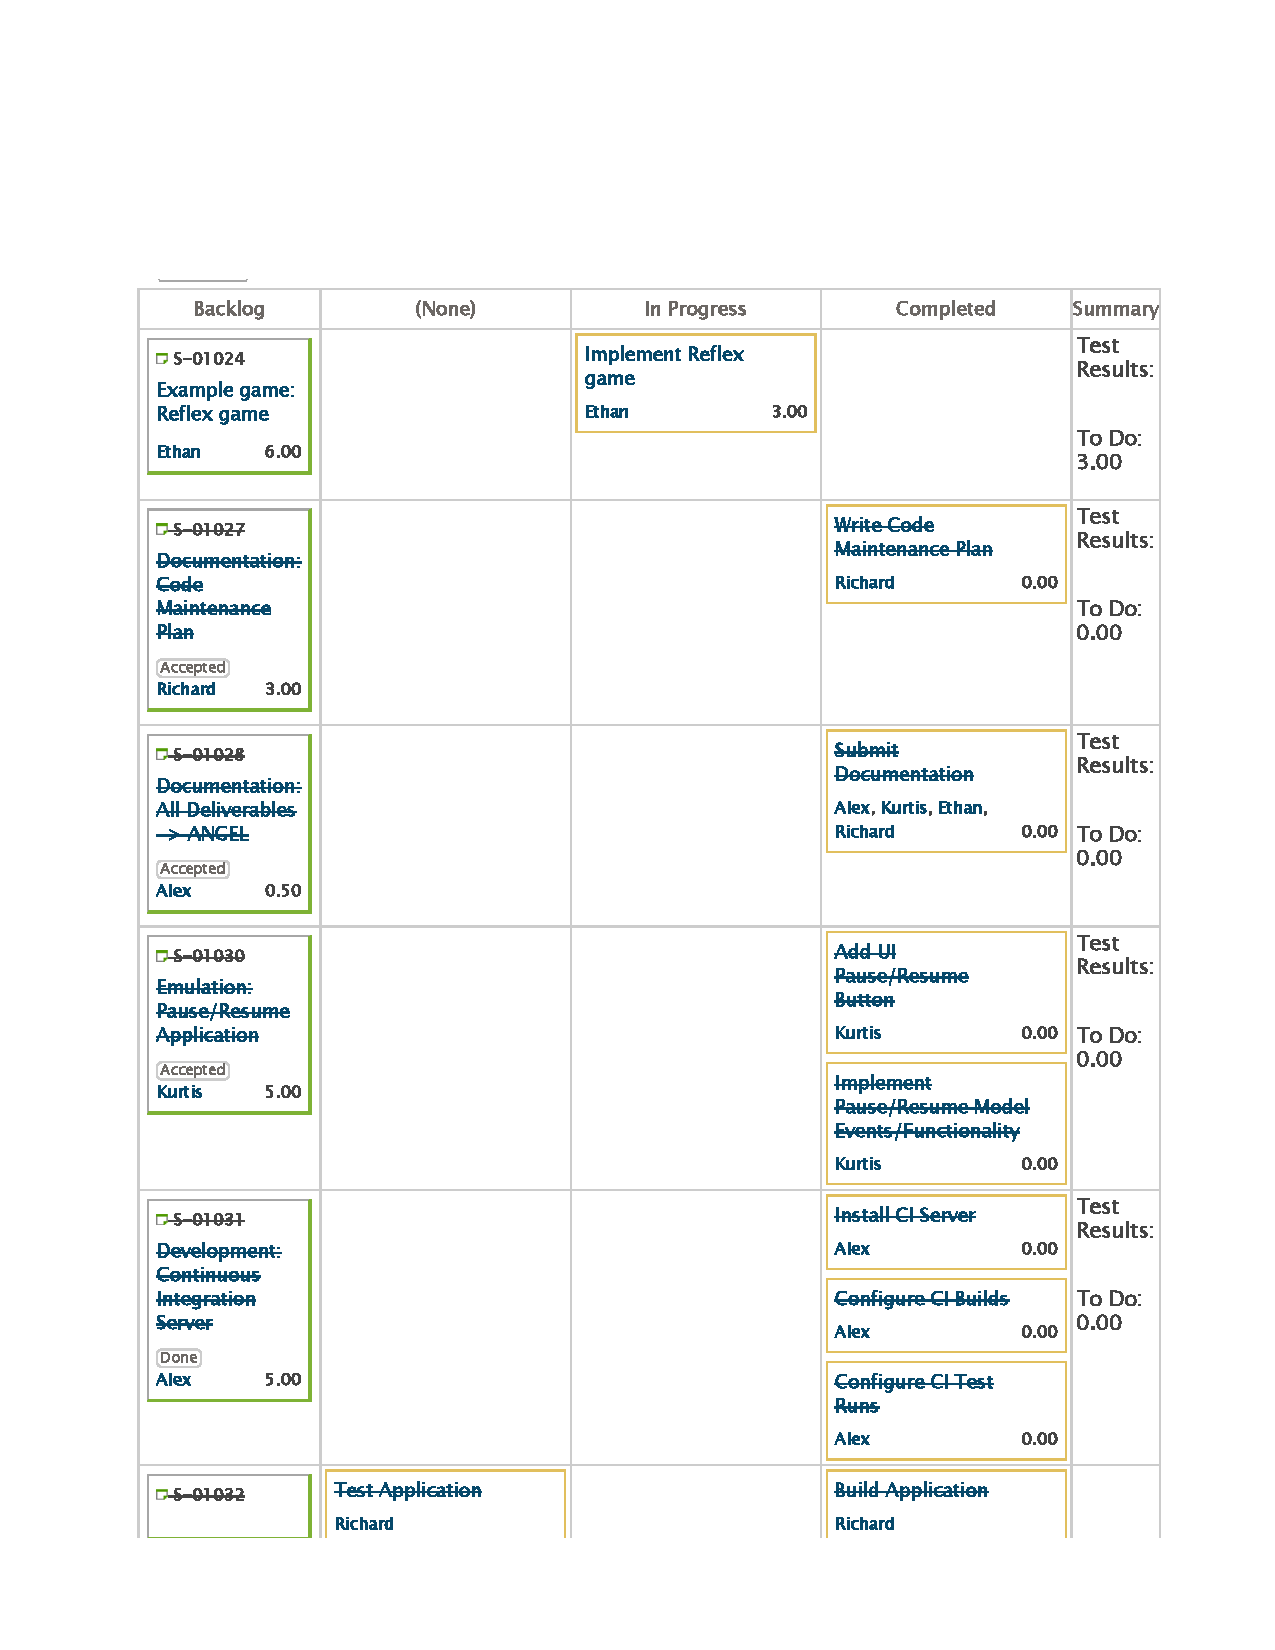
\includepdf[pages={1-2}]{pdfs/MS5VersionOne/OldSprintDetail.pdf}
        
\end{document}
